\renewcommand{\leveltopI}{-15cm + \leveltop}
\renewcommand{\leveltopII}{-15cm + \leveltopI}
\renewcommand{\leveltopIII}{-15cm + \leveltopII}
\renewcommand{\leveltopIIII}{-15cm + \leveltopIII}
\renewcommand{\leveltopIIIII}{-15cm + \leveltopIIII}
\renewcommand{\leveltopIIIIII}{-15cm + \leveltopIIIII}
\renewcommand{\leveltopIIIIIII}{-15cm + \leveltopIIIIII}
\begin{tikzpicture}[scale=.2, anchor=south]
\begin{scope}[yshift=\leveltopI cm]
\matrix (line1)[column sep=1cm] {
\node[draw=black, rectangle split,  rectangle split parts=4] (sn0x8fecef8){
\footnotesize{100}
\nodepart{two}
\begin{tikzpicture}[scale=.2]
\node[circle, scale=0.75, fill] (tid0) at (3,1.5){};
\node[circle, scale=0.75, fill] (tid1) at (2.25,3){};
\node[circle, scale=0.75, fill, red] (tid3) at (0.75,4.5){};
\node[circle, scale=0.75, fill, red] (tid4) at (2.25,4.5){};
\node[circle, scale=0.75, fill] (tid5) at (3.75,4.5){};
\draw[](tid1) -- (tid3);
\draw[](tid1) -- (tid4);
\draw[](tid1) -- (tid5);
\node[circle, scale=0.75, fill] (tid2) at (5.25,3){};
\node[circle, scale=0.75, fill, red] (tid6) at (5.25,4.5){};
\draw[](tid2) -- (tid6);
\draw[](tid0) -- (tid1);
\draw[](tid0) -- (tid2);
\end{tikzpicture}
\nodepart{three}
\footnotesize{4.37037}
\nodepart{four}
\footnotesize{$67\:33$}
};
 & 
\\
};
\end{scope}
\begin{scope}[yshift=\leveltopII cm]
\matrix (line2)[column sep=1cm] {
\node[draw=black, rectangle split,  rectangle split parts=4] (sn0x8feccd0){
\footnotesize{66.6667}
\nodepart{two}
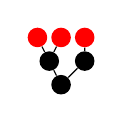
\begin{tikzpicture}[scale=.2]
\node[circle, scale=0.75, fill] (tid0) at (2.25,1.5){};
\node[circle, scale=0.75, fill] (tid1) at (1.5,3){};
\node[circle, scale=0.75, fill, red] (tid3) at (0.75,4.5){};
\node[circle, scale=0.75, fill, red] (tid4) at (2.25,4.5){};
\draw[](tid1) -- (tid3);
\draw[](tid1) -- (tid4);
\node[circle, scale=0.75, fill] (tid2) at (3.75,3){};
\node[circle, scale=0.75, fill, red] (tid5) at (3.75,4.5){};
\draw[](tid2) -- (tid5);
\draw[](tid0) -- (tid1);
\draw[](tid0) -- (tid2);
\end{tikzpicture}
\nodepart{three}
\footnotesize{4.05556}
\nodepart{four}
\footnotesize{$67\:33$}
};
 & 
\node[draw=black, rectangle split,  rectangle split parts=4] (sn0x8fee408){
\footnotesize{33.3333}
\nodepart{two}
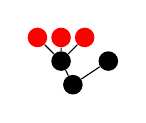
\begin{tikzpicture}[scale=.2]
\node[circle, scale=0.75, fill] (tid0) at (3,1.5){};
\node[circle, scale=0.75, fill] (tid1) at (2.25,3){};
\node[circle, scale=0.75, fill, red] (tid3) at (0.75,4.5){};
\node[circle, scale=0.75, fill, red] (tid4) at (2.25,4.5){};
\node[circle, scale=0.75, fill, red] (tid5) at (3.75,4.5){};
\draw[](tid1) -- (tid3);
\draw[](tid1) -- (tid4);
\draw[](tid1) -- (tid5);
\node[circle, scale=0.75, fill] (tid2) at (5.25,3){};
\draw[](tid0) -- (tid1);
\draw[](tid0) -- (tid2);
\end{tikzpicture}
\nodepart{three}
\footnotesize{4}
\nodepart{four}
\footnotesize{$1$}
};
 & 
\\
};
\end{scope}
\begin{scope}[yshift=\leveltopIII cm]
\matrix (line3)[column sep=1cm] {
\node[draw=black, rectangle split,  rectangle split parts=4] (sn0x8fedc20){
\footnotesize{44.4444}
\nodepart{two}
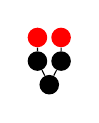
\begin{tikzpicture}[scale=.2]
\node[circle, scale=0.75, fill] (tid0) at (1.5,1.5){};
\node[circle, scale=0.75, fill] (tid1) at (0.75,3){};
\node[circle, scale=0.75, fill, red] (tid3) at (0.75,4.5){};
\draw[](tid1) -- (tid3);
\node[circle, scale=0.75, fill] (tid2) at (2.25,3){};
\node[circle, scale=0.75, fill, red] (tid4) at (2.25,4.5){};
\draw[](tid2) -- (tid4);
\draw[](tid0) -- (tid1);
\draw[](tid0) -- (tid2);
\end{tikzpicture}
\nodepart{three}
\footnotesize{3.75}
\nodepart{four}
\footnotesize{$1$}
};
 & 
\node[draw=black, rectangle split,  rectangle split parts=4] (sn0x8fee618){
\footnotesize{55.5556}
\nodepart{two}
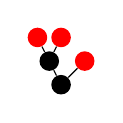
\begin{tikzpicture}[scale=.2]
\node[circle, scale=0.75, fill] (tid0) at (2.25,1.5){};
\node[circle, scale=0.75, fill] (tid1) at (1.5,3){};
\node[circle, scale=0.75, fill, red] (tid3) at (0.75,4.5){};
\node[circle, scale=0.75, fill, red] (tid4) at (2.25,4.5){};
\draw[](tid1) -- (tid3);
\draw[](tid1) -- (tid4);
\node[circle, scale=0.75, fill, red] (tid2) at (3.75,3){};
\draw[](tid0) -- (tid1);
\draw[](tid0) -- (tid2);
\end{tikzpicture}
\nodepart{three}
\footnotesize{3.66667}
\nodepart{four}
\footnotesize{$67\:33$}
};
 & 
\\
};
\end{scope}
\draw (sn0x8fecef8.south) -- (sn0x8feccd0.north);
\draw (sn0x8fecef8.south) -- (sn0x8fee408.north);
\draw (sn0x8feccd0.south) -- (sn0x8fedc20.north);
\draw (sn0x8feccd0.south) -- (sn0x8fee618.north);
\draw (sn0x8fee408.south) -- (sn0x8fee618.north);
\end{tikzpicture}

%%% Local Variables:
%%% TeX-master: "thesis/thesis.tex"
%%% End: 
\renewcommand{\leveltopI}{-15cm + \leveltop}
\renewcommand{\leveltopII}{-15cm + \leveltopI}
\renewcommand{\leveltopIII}{-15cm + \leveltopII}
\renewcommand{\leveltopIIII}{-15cm + \leveltopIII}
\renewcommand{\leveltopIIIII}{-15cm + \leveltopIIII}
\renewcommand{\leveltopIIIIII}{-15cm + \leveltopIIIII}
\renewcommand{\leveltopIIIIIII}{-15cm + \leveltopIIIIII}
\begin{tikzpicture}[scale=.2, anchor=south]
\begin{scope}[yshift=\leveltopI cm]
\matrix (line1)[column sep=1cm] {
\node[draw=black, rectangle split,  rectangle split parts=4] (sn0x8fede58){
\footnotesize{100}
\nodepart{two}
\begin{tikzpicture}[scale=.2]
\node[circle, scale=0.75, fill] (tid0) at (3,1.5){};
\node[circle, scale=0.75, fill] (tid1) at (2.25,3){};
\node[circle, scale=0.75, fill, red] (tid3) at (0.75,4.5){};
\node[circle, scale=0.75, fill, red] (tid4) at (2.25,4.5){};
\node[circle, scale=0.75, fill, red] (tid5) at (3.75,4.5){};
\draw[](tid1) -- (tid3);
\draw[](tid1) -- (tid4);
\draw[](tid1) -- (tid5);
\node[circle, scale=0.75, fill] (tid2) at (5.25,3){};
\node[circle, scale=0.75, fill] (tid6) at (5.25,4.5){};
\draw[](tid2) -- (tid6);
\draw[](tid0) -- (tid1);
\draw[](tid0) -- (tid2);
\end{tikzpicture}
\nodepart{three}
\footnotesize{4.38889}
\nodepart{four}
\footnotesize{$1$}
};
 & 
\\
};
\end{scope}
\begin{scope}[yshift=\leveltopII cm]
\matrix (line2)[column sep=1cm] {
\node[draw=black, rectangle split,  rectangle split parts=4] (sn0x8feccd0){
\footnotesize{100}
\nodepart{two}
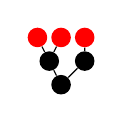
\begin{tikzpicture}[scale=.2]
\node[circle, scale=0.75, fill] (tid0) at (2.25,1.5){};
\node[circle, scale=0.75, fill] (tid1) at (1.5,3){};
\node[circle, scale=0.75, fill, red] (tid3) at (0.75,4.5){};
\node[circle, scale=0.75, fill, red] (tid4) at (2.25,4.5){};
\draw[](tid1) -- (tid3);
\draw[](tid1) -- (tid4);
\node[circle, scale=0.75, fill] (tid2) at (3.75,3){};
\node[circle, scale=0.75, fill, red] (tid5) at (3.75,4.5){};
\draw[](tid2) -- (tid5);
\draw[](tid0) -- (tid1);
\draw[](tid0) -- (tid2);
\end{tikzpicture}
\nodepart{three}
\footnotesize{4.05556}
\nodepart{four}
\footnotesize{$67\:33$}
};
 & 
\\
};
\end{scope}
\begin{scope}[yshift=\leveltopIII cm]
\matrix (line3)[column sep=1cm] {
\node[draw=black, rectangle split,  rectangle split parts=4] (sn0x8fedc20){
\footnotesize{66.6667}
\nodepart{two}
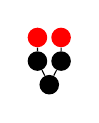
\begin{tikzpicture}[scale=.2]
\node[circle, scale=0.75, fill] (tid0) at (1.5,1.5){};
\node[circle, scale=0.75, fill] (tid1) at (0.75,3){};
\node[circle, scale=0.75, fill, red] (tid3) at (0.75,4.5){};
\draw[](tid1) -- (tid3);
\node[circle, scale=0.75, fill] (tid2) at (2.25,3){};
\node[circle, scale=0.75, fill, red] (tid4) at (2.25,4.5){};
\draw[](tid2) -- (tid4);
\draw[](tid0) -- (tid1);
\draw[](tid0) -- (tid2);
\end{tikzpicture}
\nodepart{three}
\footnotesize{3.75}
\nodepart{four}
\footnotesize{$1$}
};
 & 
\node[draw=black, rectangle split,  rectangle split parts=4] (sn0x8fee618){
\footnotesize{33.3333}
\nodepart{two}
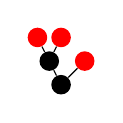
\begin{tikzpicture}[scale=.2]
\node[circle, scale=0.75, fill] (tid0) at (2.25,1.5){};
\node[circle, scale=0.75, fill] (tid1) at (1.5,3){};
\node[circle, scale=0.75, fill, red] (tid3) at (0.75,4.5){};
\node[circle, scale=0.75, fill, red] (tid4) at (2.25,4.5){};
\draw[](tid1) -- (tid3);
\draw[](tid1) -- (tid4);
\node[circle, scale=0.75, fill, red] (tid2) at (3.75,3){};
\draw[](tid0) -- (tid1);
\draw[](tid0) -- (tid2);
\end{tikzpicture}
\nodepart{three}
\footnotesize{3.66667}
\nodepart{four}
\footnotesize{$67\:33$}
};
 & 
\\
};
\end{scope}
\draw (sn0x8fede58.south) -- (sn0x8feccd0.north);
\draw (sn0x8feccd0.south) -- (sn0x8fedc20.north);
\draw (sn0x8feccd0.south) -- (sn0x8fee618.north);
\end{tikzpicture}

%%% Local Variables:
%%% TeX-master: "thesis/thesis.tex"
%%% End: 
